\documentclass[aspectratio=169]{beamer}

\usepackage[utf8]{inputenc}
\usepackage{amsmath}
\usepackage{amsfonts}
\usepackage{amssymb}
\usepackage{graphicx}
\usepackage{ragged2e}  % `\justifying` text
\usepackage{booktabs}  % Tables
\usepackage{tabularx}
\usepackage{tikz}      % Diagrams
\usetikzlibrary{calc, shapes, backgrounds}
\usepackage{dsfont}
\usepackage{url}       % `\url
\usepackage{listings}  % Code listings
\usepackage[T1]{fontenc}
\usepackage{cite}

\usepackage{theme/beamerthemehbrs}

% Define a smaller footnote size
\renewcommand{\footnotesize}{\tiny}

\author[]{Salvin George}
\title{Development of a framework for the localization of radioactive sources and evaluation methods}
% \subtitle{}
\institute[HBRS]{Hochschule Bonn-Rhein-Sieg}
\date{\today}
\subject{Test beamer}

% leave the value of this argument empty if the advisors
% should not be included on the title slide
\def\advisors{Prof. Dr. Sebastian Houben, \\Claudia Rudolph (Fraunhofer FKIE)}

% \thirdpartylogo{path/to/your/image}

\begin{document}

\begin{frame}
\titlepage
\end{frame}



% \begin{frame}
% \frametitle{Introduction}

% \begin{itemize}
%   \item Radioactivity is a fundamental aspect of life, essential for heating the Earth's core and enabling life to develop.
%   \item Radioactivity involves atoms seeking stability by emitting particles or energy.
%   \item Radioactive materials can be misused for harmful purposes, necessitating detection and securing to prevent contamination.
%   % \item Project Focus: Enhance UAV localization and path planning for detecting radioactive sources, develop a simulation and evaluation framework, compare localization methods, and address challenges like particle attenuation and scattering in detection.
%   \item Project Focus: Identify a method or combination of methods that will efficiently and accurately localize radioactive sources with minimal computational cost and also without the need for exploring the full search space.
% \end{itemize}
% \end{frame}


\begin{frame}
  \frametitle{Introduction}
  
  \begin{itemize}
    \item Historical incidents like Chernobyl (1986) and Fukushima (2011) have shown the severe impact of uncontrolled radioactive releases \cite{iaea2022itdb}.
    % \item Chernobyl released 400 times more radiation than the Hiroshima bomb, causing acute radiation syndrome and many thyroid cancer cases due to iodine-131 \cite{UNSCEAR}.
    \item Fukushima, caused by an earthquake and tsunami leading to the evacuation of over 154,000 people \cite{WHO} while Chernobyl released 400 times more radiation than the Hiroshima bomb\cite{UNSCEAR}.
    % \item Fukushima, caused by an earthquake and tsunami, released iodine-131 and cesium-137, leading to the evacuation of over 154,000 people \cite{WHO}.
    \item Detection and securing of radioactive materials are crucial to prevent misuse and contamination.
    \item \textcolor{hbrsblue}{\textbf{Project Focus:}} Develop methods to efficiently and accurately localize radioactive sources with minimal computational cost, avoiding full search space exploration.
\end{itemize}
  
  \end{frame}

% \begin{frame}
% \frametitle{Relevance of the topic}

% \begin{itemize}
  
%   % \item Since 1993, there have been 4243 confirmed incidents of radioactive materials being lost or stolen, with 52\% occurring during authorized transports.
%   % \item It is also worth noting that 87\% of the theft incidents for malicious intents remain undetected. \{Source: IAEA Incident and Trafficking Database}
%   % \item Therefore, the necessity for a tool that helps to source the radioactive materials is of utmost importance.
% \end{itemize}
% \end{frame}


\begin{frame}
  \frametitle{Relevance of the topic}
  
  \begin{columns}
    \begin{column}{0.5\textwidth}
      \begin{itemize}
        \item The results of this project will be beneficial to the security agencies and law enforcement agencies to detect the radioactive sources in a timely manner.
        \item This localization of the radioactive sources can be useful to the nuclear power plants to detect the leakages in the reactor.
        \item Localizing the radioactive sources prevents the contamination of the environment and the food chain.
      \end{itemize}
  
    \end{column}
    \begin{column}{0.5\textwidth}
      \begin{figure}
        \centering
        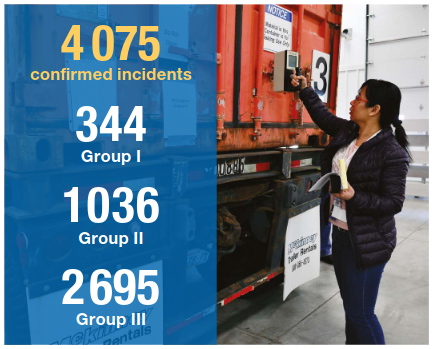
\includegraphics[width=0.8\textwidth]{images/radi_incidents2.png}
        \caption{The number of the incidents recorded in ITDB during the period 1993-2022 per incident type group. \cite{iaea2022itdb}}
        \label{fig:Relevance}
      \end{figure}
    \end{column}
  \end{columns}
    
  \end{frame}


% \begin{frame}
%   \frametitle{Relevance - Continued}

%   \begin{figure}
%     \centering
%     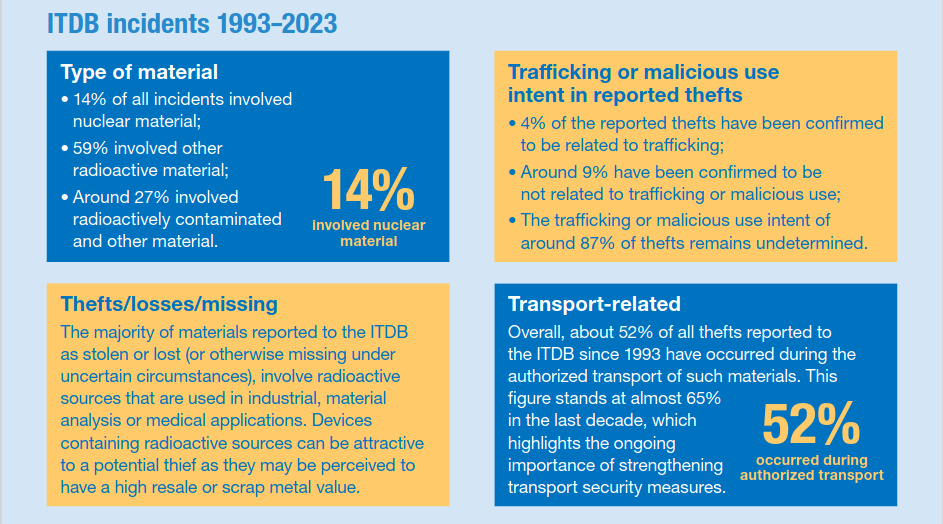
\includegraphics[width=0.8\textwidth]{images/relevance.png}
%     \caption{Incidents of Radioactive Material Loss or Theft}
%     \label{fig:IAEA}
%   \end{figure}
%   % \{Source: IAEA Incident and Trafficking Database}
% \end{frame}

% \begin{frame}
% \frametitle{Related works}
% \begin{itemize}
%   \item Dual-Stage Planner for Autonomous Radioactive Source Localization in Unknown Environments \cite{zhu2024dual}
%   \begin{itemize}
%     \item Two-stage process: Source Tracking and Relocation.
%     \item Utilizes convex polyhedrons for complex environments.
%     \item High success rate with fewer measurements.
%   \end{itemize}
%   \item Adaptive Bayesian Sensor Motion Planning for Hazardous Source Term Reconstruction \cite{hutchinson2017adaptive}
%   \begin{itemize}
%     \item Uses Markov Chain Monte Carlo for source parameter estimation.
%     \item Selects maneuvers based on maximum entropy sampling.
%   \end{itemize}
%   \item Airborne Radiation Mapping: Overview and Application of Current and Future Aerial Systems \cite{connor2016airborne}
%   \begin{itemize}
%     \item Utilizes UAVs for rapid area mapping.
%     \item Effective for radiation detection from aerial platforms.
%   \end{itemize} 
% \end{itemize}
% \end{frame}

% \begin{frame}
% \frametitle{Related works: continued}
% \begin{itemize}
%   \item Particle Filter Based Information-Theoretic Active Sensing \cite{ryan2010particle}
%   \begin{itemize}
%     \item Employs particle filters for estimating target locations.
%     \item Minimizes entropy over a receding horizon.
%   \end{itemize}
%   \item Detection and Localization of Hidden Radioactive Sources with Spatial Statistical Method \cite{wan2012detection}
%   \begin{itemize}
%     \item Uses spatial statistical methods and Poisson distribution models.
%     \item Effective in various environmental conditions.
%   \end{itemize}
%   \item Path Planning Algorithm Ensuring Accurate Localization of Radiation Sources \cite{woller2022path}
%   \begin{itemize}
%     \item Combines UAV and UGV for fast mapping and accurate localization.
%     \item Uses Generalized Travelling Salesman Problem (GTSP) solver.
%     \item Minimizes total path length while ensuring accurate source localization.
%   \end{itemize}


% \end{itemize}
% \end{frame}


% \begin{frame}
%   \frametitle{Related Work}
%   \begin{itemize}
%     \item Rollout Algorithm \footnote{Hoffmann, Folker, et al. "A rollout based path planner for emitter localization." 2019 22th International Conference on Information Fusion (FUSION). IEEE, 2019.}
%     \item Entropy Algorithm \footnote{Zhu, Hongbiao, et al. "A novel odor source localization system based on particle filtering and information entropy." Robotics and autonomous systems 132 (2020): 103619}
%     \item Gradient Descent \footnote{Wu, Yizhi, et al. "Convolutionally evaluated gradient first search path planning algorithm without prior global maps." Robotics and Autonomous Systems 150 (2022): 103985.}
%     % \item 
%   \end{itemize}
% \end{frame}



% \begin{frame}
%   \frametitle{Related Work}

%   \begin{columns}
%     \begin{column}{0.3\textwidth}
%       \begin{itemize}
%         \item Rollout Algorithm \footnote{Hoffmann, Folker, et al. "A rollout based path planner for emitter localization." 2019 22th International Conference on Information Fusion (FUSION). IEEE, 2019.}
%         \item Entropy Algorithm \footnote{Zhu, Hongbiao, et al. "A novel odor source localization system based on particle filtering and information entropy." Robotics and autonomous systems 132 (2020): 103619}
%         \item Gradient Descent \footnote{Wu, Yizhi, et al. "Convolutionally evaluated gradient first search path planning algorithm without prior global maps." Robotics and Autonomous Systems 150 (2022): 103985.}
%       \end{itemize}
%     \end{column}

%     \begin{column}{0.7\textwidth}
%       \begin{figure}
%         \centering
%         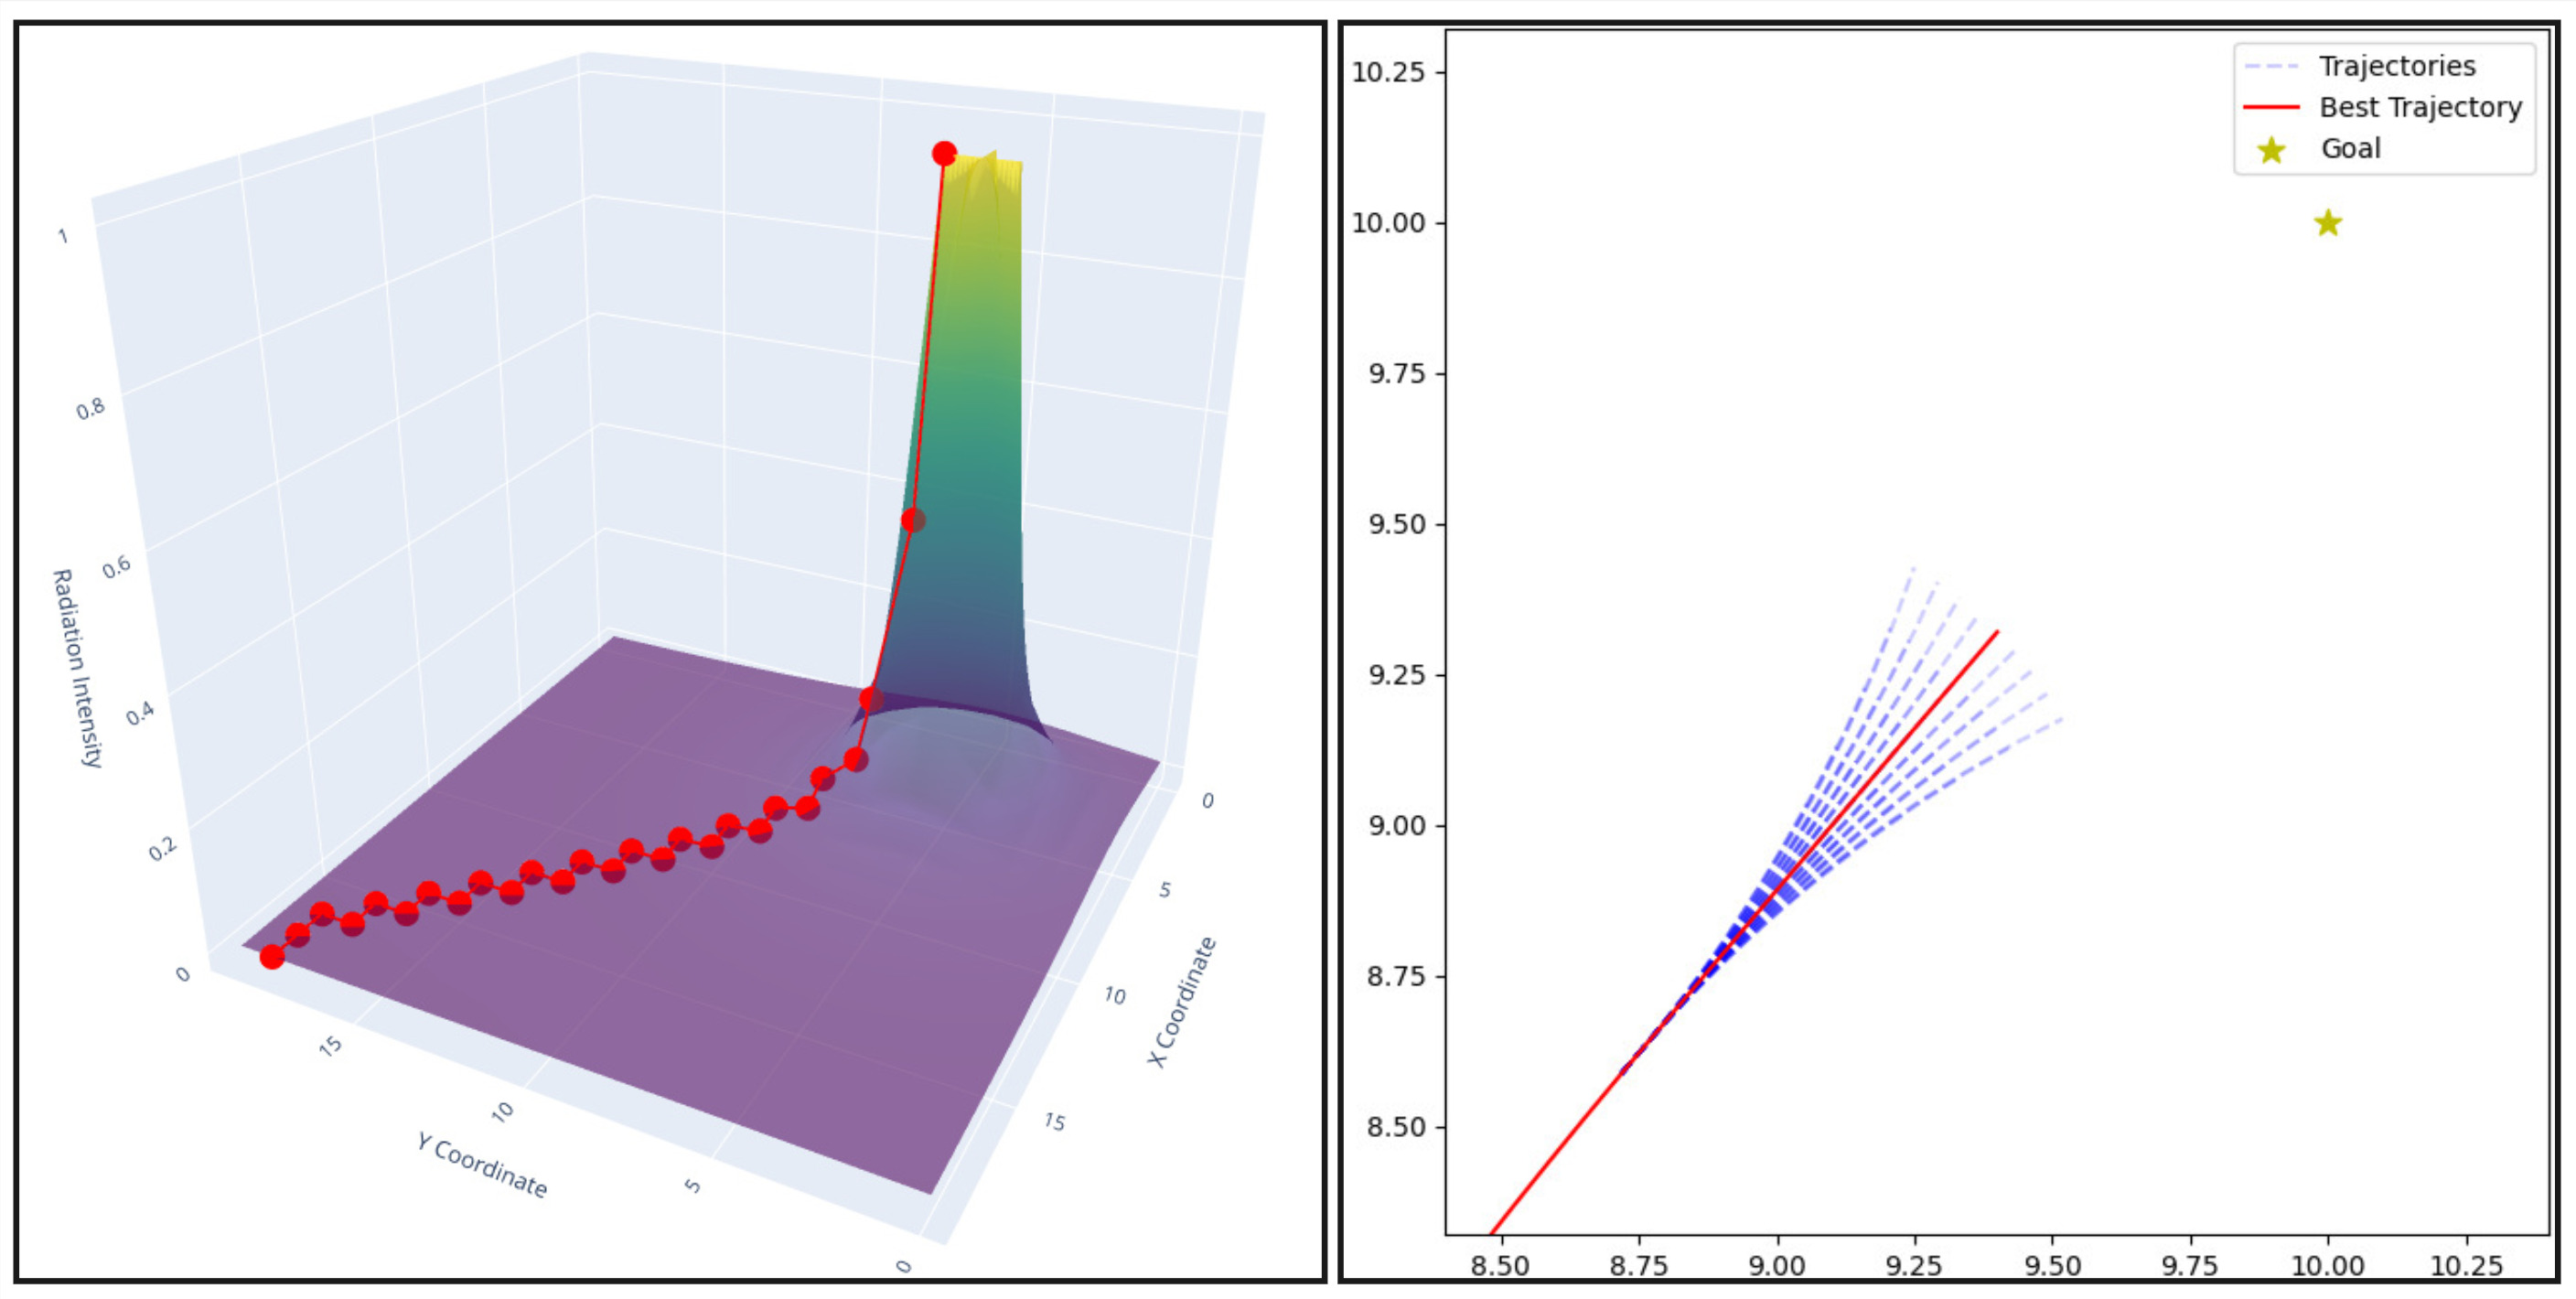
\includegraphics[width=\textwidth]{images/related_work.jpg}
%         \caption{Your Image Description}
%       \end{figure}
%     \end{column}
%   \end{columns}
% \end{frame}





% \begin{frame}
% \frametitle{Deficiencies of the current approaches}
% \begin{itemize}
%   \item High Computational Cost and scalability: Many methods require significant computational resources, challenging real-time applications and not easily scalable to large environments. \cite{zhu2024dual} \cite{hutchinson2017adaptive} \cite{ryan2010particle}
%   % \item Complexity in Dynamic Environments: Adapting to highly dynamic and unpredictable environments remains difficult.
%   % \item Dependency on Training Data: Reinforcement learning methods need extensive and accurate training data, which can be difficult to obtain.
%   \item Hardware Limitations: UAV-based methods are constrained by battery life, weather conditions, and hardware capabilities. \cite{connor2016airborne} \cite{woller2022path}
%   % \item Scalability Issues: Some methods are not easily scalable to large or complex environments due to their inherent computational demands.
%   \item Real-Time Applicability: Achieving real-time performance while maintaining accuracy and reliability is a common challenge across many methods. \cite{zhu2024dual} \cite{ryan2010particle} \cite{woller2022path}
%   \item Exploring full search space: Many methods explore the full search space, leading to high exploration time and cost. \cite{woller2022path} \cite{connor2016airborne}
% \end{itemize}
% \end{frame}


\begin{frame}
  \frametitle{Deficiencies of the current approaches}
  \begin{itemize}
    \item Many methods are significantly \textcolor{hbrsblue}{\textbf{computationally expensive}}, and easily \textcolor{hbrsblue}{\textbf{not scalable}} to large environments. \cite{zhu2024dual} \cite{hutchinson2017adaptive} \cite{ryan2010particle}
    % \item Complexity in Dynamic Environments: Adapting to highly dynamic and unpredictable environments remains difficult.
    % \item Dependency on Training Data: Reinforcement learning methods need extensive and accurate training data, which can be difficult to obtain.
    \item UAV-based methods are constrained by \textcolor{hbrsblue}{\textbf{hardware limitations}}, for example, battery life, weather conditions, and hardware capabilities. \cite{connor2016airborne} \cite{woller2022path}
    % \item Scalability Issues: Some methods are not easily scalable to large or complex environments due to their inherent computational demands.
    \item Achieving \textcolor{hbrsblue}{\textbf{real-time performance}} while maintaining accuracy and reliability is a common challenge across many methods. \cite{zhu2024dual} \cite{ryan2010particle} \cite{woller2022path}
    \item Many methods explore the \textcolor{hbrsblue}{\textbf{full search space}}, leading to high exploration time and cost. \cite{woller2022path} \cite{connor2016airborne}
  \end{itemize}
  \end{frame}



\begin{frame}
  \frametitle{Related Work}
  
  \begin{columns}
    \begin{column}{0.4\textwidth}
      \begin{itemize}
        \item Rollout Algorithm \cite{hoffmann2019rollout}%\footnote{Hoffmann, Folker, et al. "A rollout based path planner for emitter localization." 2019 22th International Conference on Information Fusion (FUSION). IEEE, 2019.}
        \item Entropy Algorithm \cite{zhu2020novel}%\footnote{Zhu, Hongbiao, et al. "A novel odor source localization system based on particle filtering and information entropy." Robotics and autonomous systems 132 (2020): 103619}
        \item Gradient Descent \cite{wu2022convolutionally}%\footnote{Wu, Yizhi, et al. "Convolutionally evaluated gradient first search path planning algorithm without prior global maps." Robotics and Autonomous Systems 150 (2022): 103985.}
        \item Spatial Statistical Method \cite{wan2012detection}
        \item Principle Component Analysis \cite{kishimoto2021path}
      \end{itemize}
    \end{column}
    \begin{column}{0.6\textwidth}
      \begin{figure}
        \centering
        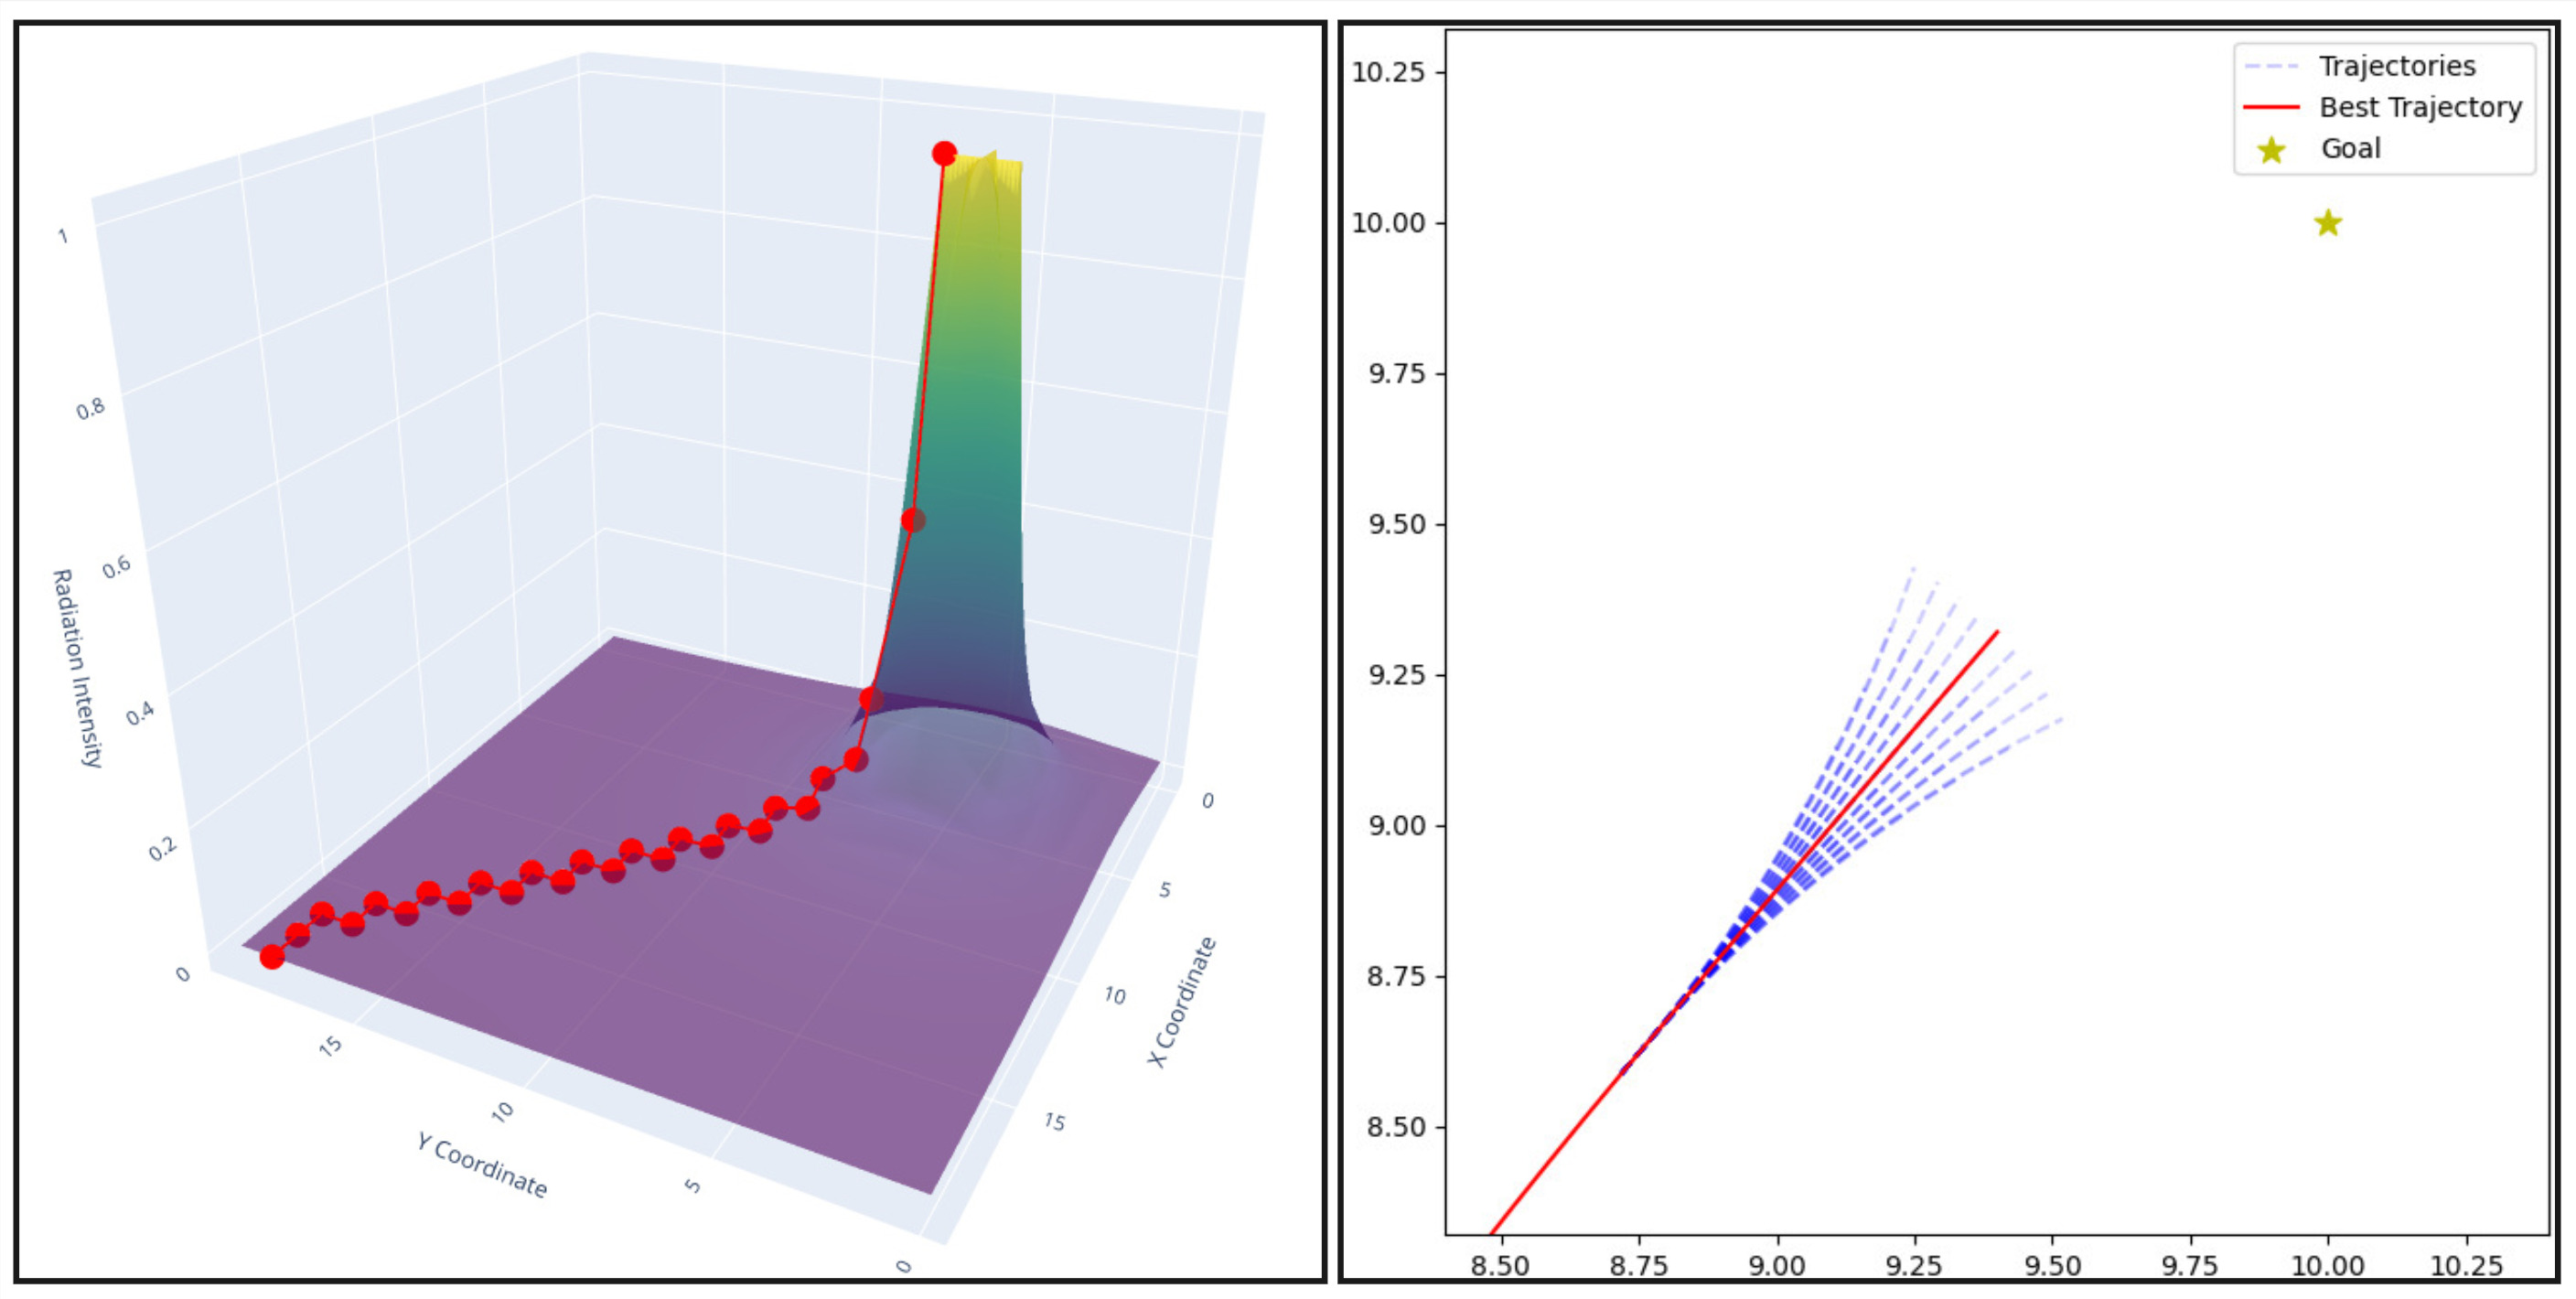
\includegraphics[width=0.8\textwidth]{images/related_work.jpg}
        \caption{Gradient Descent Algorithm(left) and Rollout Algorithm (right)}
        \label{fig:Relevance}
      \end{figure}
    \end{column}
  \end{columns}
    
\end{frame}

\begin{frame}
  \frametitle{Proposed approach}
  

  \begin{itemize}
    \item Enhance localization and path planning for UAVs to detect radioactive sources.
    \item Develop simulation and evaluation framework for radioactive sources.
    \item Evaluate and compare different methods for radioactive source localization.
    \item Address challenges such as particle attenuation and scattering in detection methods.
  \end{itemize}
  % \begin{columns}
  %   \begin{column}{0.5\textwidth}
      
  
  %   \end{column}
  %   \begin{column}{0.5\textwidth}

  %     \begin{figure}
  %       \centering
  %       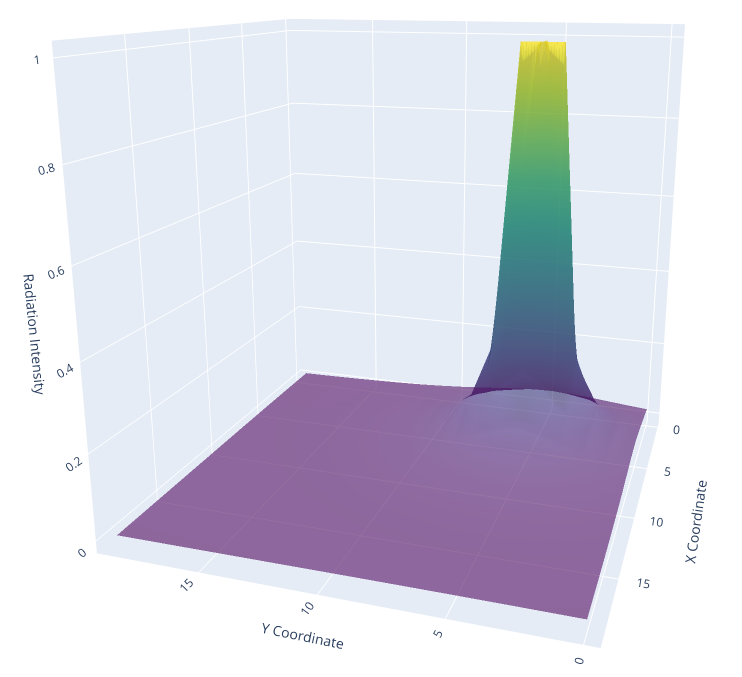
\includegraphics[width=0.8\textwidth]{images/radiation_distribution.png}
  %       \caption{Single source radiation distribution in an environment}
  %       \label{fig:approach}
  %     \end{figure}
  
  %   \end{column}
  % \end{columns}
    
\end{frame}

\begin{frame}
\frametitle{Work Plan}
\begin{figure}
  \centering
  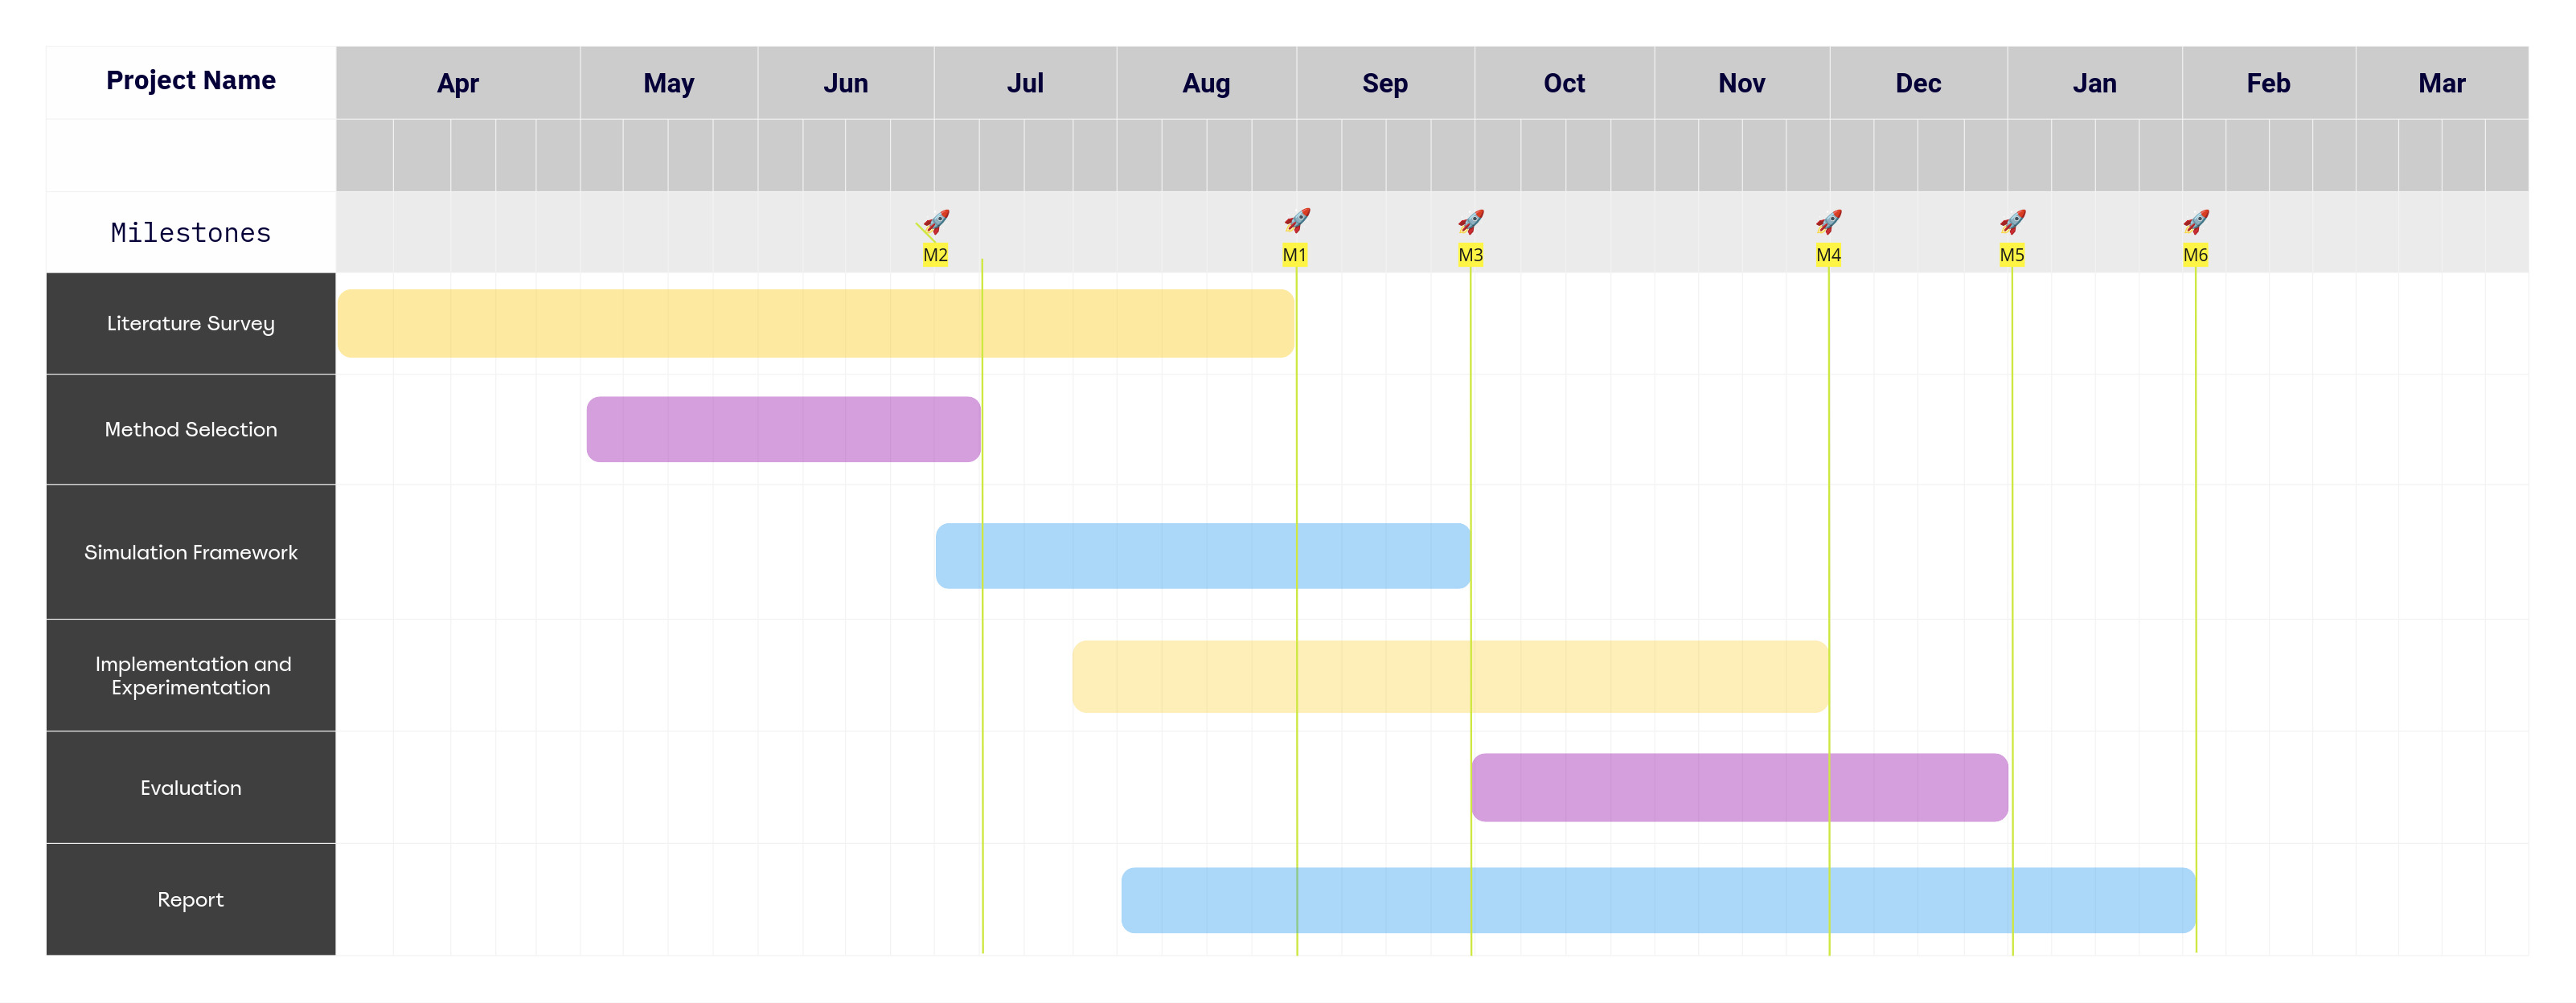
\includegraphics[width=1\textwidth]{images/work_plan.jpg}
  \caption{Work Plan}
  \label{fig:work_plan}
\end{figure}
\end{frame}


\bibliography{references}
\bibliographystyle{plain}

\end{document}
